\documentclass{article}

\usepackage{cancel}
\usepackage{algorithm} %pseudo-code
\usepackage{algpseudocode}
\usepackage[columnsep=1cm, top=1cm, bottom=1.5cm, left=1cm, right=1cm]{geometry}
\usepackage{amsmath,amsthm,amssymb}
\usepackage{graphicx}
\usepackage{float}
\usepackage{amsmath, amssymb, amscd}
\usepackage{alltt}
\usepackage{textcomp}
\usepackage{gensymb}
\usepackage{multicol}
\usepackage{tabularx}
\usepackage{units}
%\usepackage{mathpple}
%\usepackage{mathpazo}
\usepackage{fouriernc}
%\usepackage{euler}
\usepackage[mathscr]{euscript}

\newcommand{\N}{\mathbb{N}}
\newcommand{\Z}{\mathbb{Z}}
\newcommand{\R}{\mathbb{R}}
\newcommand{\bigo}{\mathcal{O}}
\newcommand{\G}{\mathcal{G}}
\newcommand{\V}{\mathcal{V}}
\newcommand{\E}{\mathcal{E}}
\newcommand{\K}{\mathcal{K}}
\newcommand{\T}{^\intercal}

\def\changemargin#1#2{\list{}{\rightmargin#2\leftmargin#1}\item[]}
\let\endchangemargin=\endlist 

\newcommand{\sups}[1]{\ensuremath{^{\textrm{#1}}}}
\newcommand{\subs}[1]{\ensuremath{_{\textrm{#1}}}}

\newcommand{\specialcell}[2][c]
{
  \begin{tabular}[#1]{@{}c@{}}#2\end{tabular}
}

\makeatletter
\newsavebox{\mybox}\newsavebox{\mysim}
\newcommand{\distras}[1]
{
  \savebox{\mybox}{\hbox{\kern3pt$\scriptstyle#1$\kern3pt}}%
  \savebox{\mysim}{\hbox{$\sim$}}%
  \mathbin{\overset{#1}{\kern\z@\resizebox{\wd\mybox}{\ht\mysim}{$\sim$}}}%
}
\makeatother

% aligned matrix negative signs:
\makeatletter
\renewcommand*\env@matrix[1][c]{\hskip -\arraycolsep
  \let\@ifnextchar\new@ifnextchar
  \array{*\c@MaxMatrixCols #1}}
\makeatother

%===============================================================================
% code highlighting :
\usepackage{listings}

% define custom colors :
\usepackage{color}
\definecolor{bg}{rgb}{0.96,0.96,0.85}
\definecolor{deepblue}{rgb}{0,0,0.5}
\definecolor{deepred}{rgb}{0.6,0,0}
\definecolor{deepgreen}{rgb}{0,0.5,0}

\usepackage{xcolor}
\renewcommand{\lstlistlistingname}{Code Listings}
\renewcommand{\lstlistingname}{Code Listing}
\definecolor{gray}{gray}{0.5}
\colorlet{commentcolour}{green!50!black}

\colorlet{stringcolour}{red!60!black}
\colorlet{keywordcolour}{magenta!90!black}
\colorlet{exceptioncolour}{yellow!50!red}
\colorlet{commandcolour}{blue!60!black}
\colorlet{numpycolour}{blue!60!green}
\colorlet{literatecolour}{magenta!90!black}
\colorlet{promptcolour}{green!50!black}
\colorlet{specmethodcolour}{violet}
\colorlet{indendifiercolour}{green!70!white}

\newcommand{\framemargin}{5ex}

\newcommand{\literatecolour}{\textcolor{literatecolour}}

\newcommand\Small{\fontsize{1.00}{5.0}\selectfont}

\newcommand\pythonstyle{\lstset{
%keepspaces=true,
language=python,
showtabs=true,
tab=,
tabsize=2,
basicstyle=\ttfamily\Small,%\setstretch{.5},
stringstyle=\color{stringcolour},
showstringspaces=false,
alsoletter={1234567890},
otherkeywords={\ , \}, \{, \%, \&, \|},
keywordstyle=\color{keywordcolour}\bfseries,
emph={and,break,class,continue,def,yield,del,elif ,else,%
except,exec,finally,for,from,global,if,import,in,%
lambda,not,or,pass,print,raise,return,try,while,assert},
emphstyle=\color{blue}\bfseries,
emph={[2]True, False, None},
emphstyle=[2]\color{keywordcolour},
emph={[3]object,type,isinstance,copy,deepcopy,zip,enumerate,reversed,list,len,dict,tuple,xrange,append,execfile,real,imag,reduce,str,repr},
emphstyle=[3]\color{commandcolour},
emph={Exception,NameError,IndexError,SyntaxError,TypeError,ValueError,OverflowError,ZeroDivisionError},
emphstyle=\color{exceptioncolour}\bfseries,
%upquote=true,
morestring=[s]{"""}{"""},
morestring=[s]{'''}{'''},
commentstyle=\color{commentcolour}\slshape,
%emph={[4]1, 2, 3, 4, 5, 6, 7, 8, 9, 0},
emph={[4]ode, fsolve, sqrt, exp, sin, cos, arccos, pi,  array, norm, solve, dot, arange, , isscalar, max, sum, flatten, shape, reshape, find, any, all, abs, linspace, legend, quad, polyval,polyfit, hstack, concatenate,vstack,column_stack,empty,zeros,ones,rand,vander,grid,pcolor,eig,eigs,eigvals,svd,qr,tan,det,logspace,roll,min,mean,cumsum,cumprod,diff,vectorize,lstsq,cla,eye,xlabel,ylabel,squeeze,plot,median,std,hist},
emphstyle=[4]\color{numpycolour},
emph={[5]__init__,__add__,__mul__,__div__,__sub__,__call__,__getitem__,__setitem__,__eq__,__ne__,__nonzero__,__rmul__,__radd__,__repr__,__str__,__get__,__truediv__,__pow__,__name__,__future__,__all__},
emphstyle=[5]\color{specmethodcolour},
emph={[6]assert,range,yield},
emphstyle=[6]\color{keywordcolour}\bfseries,
% emph={[7]self},
% emphstyle=[7]\bfseries,
literate=*%
{:}{{\literatecolour:}}{1}%
{=}{{\literatecolour=}}{1}%
{-}{{\literatecolour-}}{1}%
{+}{{\literatecolour+}}{1}%
{*}{{\literatecolour*}}{1}%
{/}{{\literatecolour/}}{1}%
{!}{{\literatecolour!}}{1}%
%{(}{{\literatecolour(}}{1}%
%{)}{{\literatecolour)}}{1}%
{[}{{\literatecolour[}}{1}%
{]}{{\literatecolour]}}{1}%
{<}{{\literatecolour<}}{1}%
{>}{{\literatecolour>}}{1}%
{>>>}{{\textcolor{promptcolour}{>>>}}}{1}%
,%
breaklines=true,
breakatwhitespace= true,
%xleftmargin=\framemargin,
%xrightmargin=\framemargin,
aboveskip=1ex,
frame=trbl,
%frameround=tttt,
rulecolor=\color{black!40},
%framexleftmargin=\framemargin,
%framextopmargin=.1ex,
%framexbottommargin=.1ex,
%framexrightmargin=\framemargin,
%framexleftmargin=1mm, framextopmargin=1mm, frame=shadowbox, rulesepcolor=\color{blue},#1
%frame=tb,
backgroundcolor=\color{yellow!10}
}}

\newcommand\Rstyle{\lstset{
%keepspaces=true,
language=R,
showtabs=true,
tab=,
tabsize=2,
basicstyle=\ttfamily\Small,%\setstretch{.5},
stringstyle=\color{stringcolour},
showstringspaces=false,
alsoletter={1234567890},
otherkeywords={\ , \}, \{, \%, \&, \|},
keywordstyle=\color{keywordcolour}\bfseries,
emph={and,break,class,continue,def,yield,del,elif ,else,%
except,exec,finally,for,from,global,if,import,in,%
lambda,not,or,pass,print,raise,return,try,while,assert},
emphstyle=\color{blue}\bfseries,
emph={[2]True, False, None},
emphstyle=[2]\color{keywordcolour},
emph={[3]object,type,isinstance,copy,deepcopy,zip,enumerate,reversed,list,len,dict,tuple,xrange,append,execfile,real,imag,reduce,str,repr},
emphstyle=[3]\color{commandcolour},
emph={Exception,NameError,IndexError,SyntaxError,TypeError,ValueError,OverflowError,ZeroDivisionError},
emphstyle=\color{exceptioncolour}\bfseries,
%upquote=true,
morestring=[s]{"""}{"""},
morestring=[s]{'''}{'''},
commentstyle=\color{commentcolour}\slshape,
%emph={[4]1, 2, 3, 4, 5, 6, 7, 8, 9, 0},
emph={[4]ode, fsolve, sqrt, exp, sin, cos, arccos, pi,  array, norm, solve, dot, arange, , isscalar, max, sum, flatten, shape, reshape, find, any, all, abs, linspace, legend, quad, polyval,polyfit, hstack, concatenate,vstack,column_stack,empty,zeros,ones,rand,vander,grid,pcolor,eig,eigs,eigvals,svd,qr,tan,det,logspace,roll,min,mean,cumsum,cumprod,diff,vectorize,lstsq,cla,eye,xlabel,ylabel,squeeze,plot,median,std,hist},
emphstyle=[4]\color{numpycolour},
emph={[5]__init__,__add__,__mul__,__div__,__sub__,__call__,__getitem__,__setitem__,__eq__,__ne__,__nonzero__,__rmul__,__radd__,__repr__,__str__,__get__,__truediv__,__pow__,__name__,__future__,__all__},
emphstyle=[5]\color{specmethodcolour},
emph={[6]assert,range,yield},
emphstyle=[6]\color{keywordcolour}\bfseries,
% emph={[7]self},
% emphstyle=[7]\bfseries,
literate=*%
{:}{{\literatecolour:}}{1}%
{=}{{\literatecolour=}}{1}%
{-}{{\literatecolour-}}{1}%
{+}{{\literatecolour+}}{1}%
{*}{{\literatecolour*}}{1}%
{/}{{\literatecolour/}}{1}%
{!}{{\literatecolour!}}{1}%
%{(}{{\literatecolour(}}{1}%
%{)}{{\literatecolour)}}{1}%
{[}{{\literatecolour[}}{1}%
{]}{{\literatecolour]}}{1}%
{<}{{\literatecolour<}}{1}%
{>}{{\literatecolour>}}{1}%
{>>>}{{\textcolor{promptcolour}{>>>}}}{1}%
,%
breaklines=true,
breakatwhitespace= true,
%xleftmargin=\framemargin,
%xrightmargin=\framemargin,
aboveskip=1ex,
frame=trbl,
%frameround=tttt,
rulecolor=\color{black!40},
%framexleftmargin=\framemargin,
%framextopmargin=.1ex,
%framexbottommargin=.1ex,
%framexrightmargin=\framemargin,
%framexleftmargin=1mm, framextopmargin=1mm, frame=shadowbox, rulesepcolor=\color{blue},#1
%frame=tb,
backgroundcolor=\color{yellow!10}
}}

% Python environment
\lstnewenvironment{python}[1][]
{
  \pythonstyle
  \lstset{#1}
}
{}

% R environment
\lstnewenvironment{Rs}[1][]
{
  \Rstyle
  \lstset{#1}
}
{}

% Python for external files
\newcommand\pythonexternal[1]
{{
  \pythonstyle
  \lstinputlisting{#1}
}}

% R for external files
\newcommand\Rexternal[1]
{{
  \Rstyle
  \lstinputlisting{#1}
}}

% Python for inline
\newcommand\pythoninline[1]
{{
  \pythonstyle
  \lstinline!#1!
}}

% answer box :
\newcommand\answer[1]
{{
  \begin{center}
    \parbox[t]{5in}{#1}
  \end{center}
}}

% end code highlighting
%===============================================================================


% border matrix with brackets :
\usepackage{etoolbox}
\let\bbordermatrix\bordermatrix
\patchcmd{\bbordermatrix}{8.75}{4.75}{}{}
\patchcmd{\bbordermatrix}{\left(}{\left[}{}{}
\patchcmd{\bbordermatrix}{\right)}{\right]}{}{}


\begin{document}
\footnotesize

\title{Clustering}
\author{Evan Cummings\\
CSCI 548 -- Douglas W.~Raiford -- Pattern Recognition}

\maketitle

\section{``Smiley'' data :}

\subsection{$k$-means clustering :}

\begin{figure}[H]
  \centering
    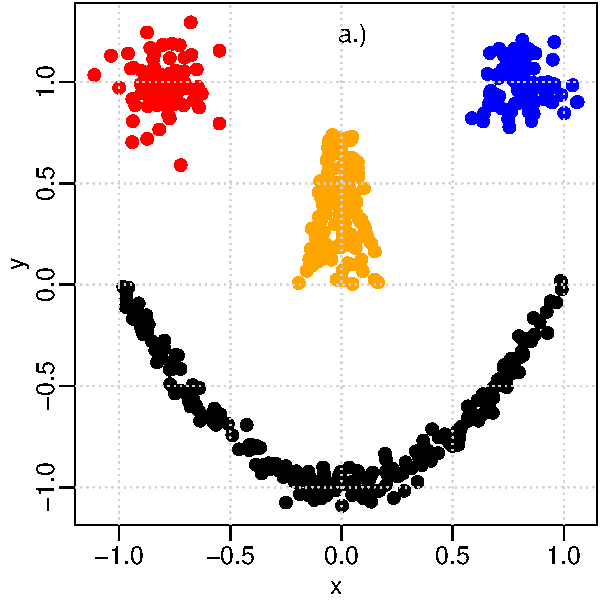
\includegraphics[width=0.28\textwidth]{images/actual_smiley.pdf}
    \quad
    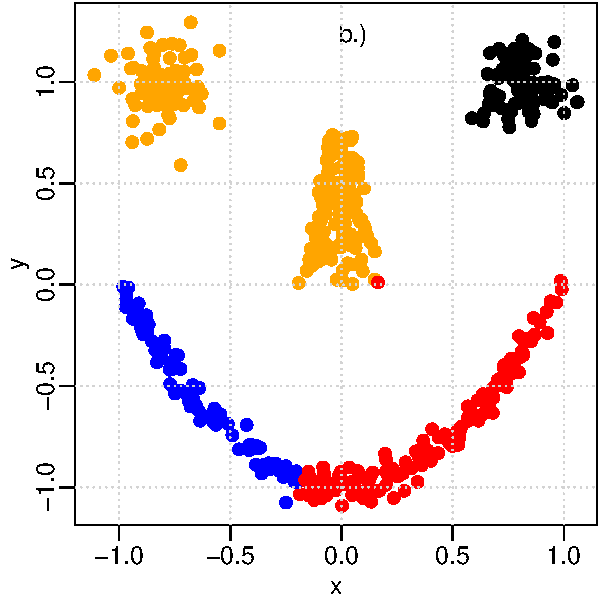
\includegraphics[width=0.28\textwidth]{images/kmeans_smiley.pdf}
    \quad
    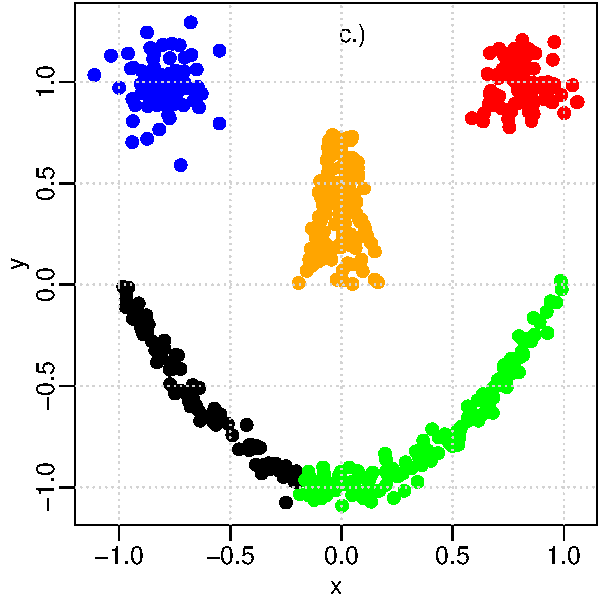
\includegraphics[width=0.28\textwidth]{images/kmeans_5_smiley.pdf}
  \caption{The original Smiley data (left) with types left eye, right eye, nose, and mouth colored arbitrarily; the $k$-means-derived classes with $k=4$ (middle); and the $k$-means-derived classes with $k=5$ (right). Note that $k$-means seeks to find $k$ clusters with minimum within-cluster-sum-of-distances from the cluster-center squared, and hence splits the data halfway between cluster means.  Because these data include a cluster, the `mouth', with an $x$-mean identical to the `nose' and directly in-between the two `eyes', $k$-means performed over these data with $k=4$ splits the `mouth' in two and assigns the `nose' cluster to one of the other `eye' clusters.  The phenomenon is further illustrated with the $k=5$ data (right) which displays five somewhat-equally-sized regions around the five cluster means.} 
\end{figure}

\subsection{hierarchical clustering :}

\begin{figure}[H]
  \centering
    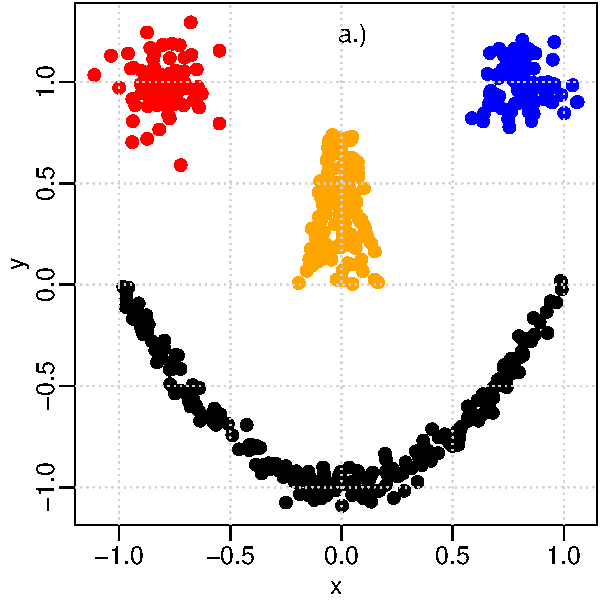
\includegraphics[width=0.28\textwidth]{images/actual_smiley.pdf}
    \quad
    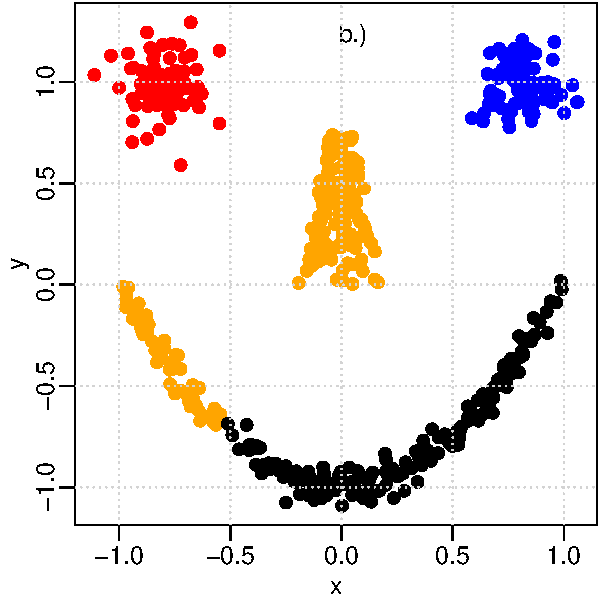
\includegraphics[width=0.28\textwidth]{images/hierClust_smiley.pdf}
    \quad
    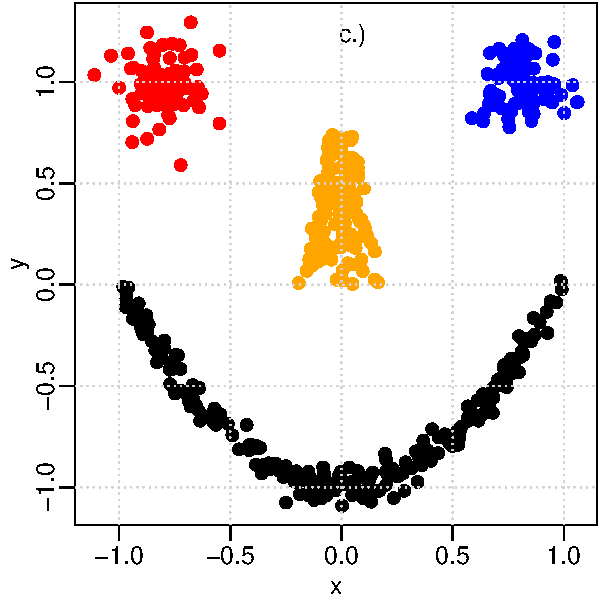
\includegraphics[width=0.28\textwidth]{images/hierClust_ward_smiley.pdf}
  \caption{The original Smiley data (left) with types left eye, right eye, nose, and mouth colored arbitrarily; clusters obtained by using hierarchical clustering with the \emph{complete linkage} method (middle); and hierarchical clustering performed with the \emph{Ward} method (right).  The complete linkage method combines clusters with minimum distance to each other, while the Ward method combines clusters which minimizes the total within-cluster variance, or \emph{error sum of squares}.  Because these data include highly-separated clusters, the Ward method is appropriate.}
\end{figure}

\newpage

\subsection{R source code :}

\begin{multicols*}{2}

\Rexternal{../src/smiley.r}

\end{multicols*}

\newpage

\section{Sequential-forward algorithm applied to the ``Iris'' data :}

\begin{figure}[H]
  \centering
    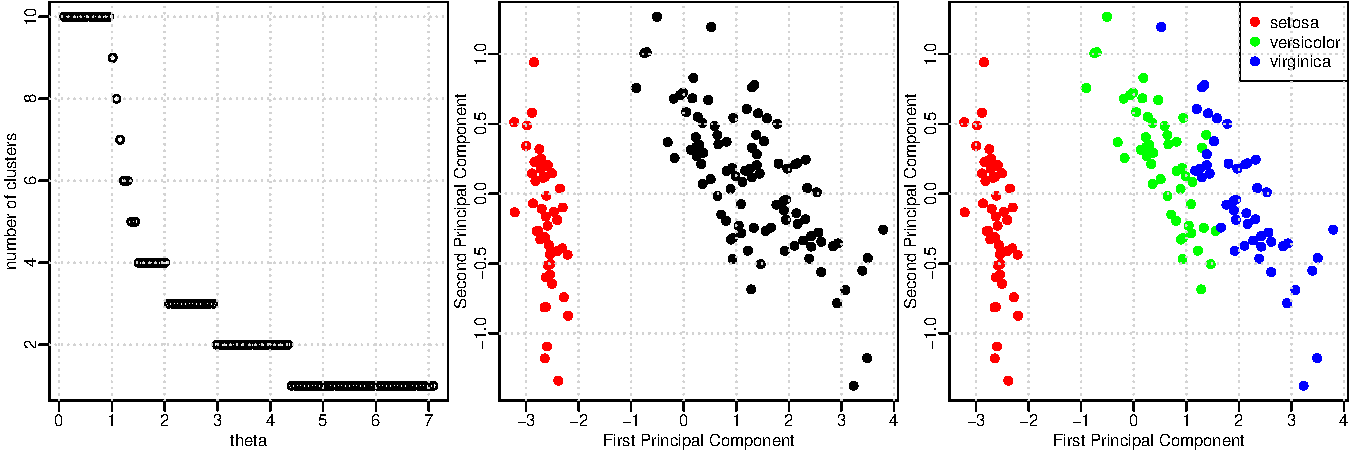
\includegraphics[width=0.95\textwidth]{images/iris_clusters.pdf}
  \caption{The number of clusters derived with a given characteristic distance for the \emph{Iris} data using sequential clustering (left), the optimal clustering for $\hat{\theta}=3.5$ (middle), and data plotted by class (right).  Here, $\hat{\theta}$ was chosen as being representative of the most prevalent $\theta$-value corresponding to a number of clusters greater than one.  Note that while the Iris data contains three distinct classes, two of them are very close together.   Due to the fact that the sequential-forward algorithm combines nearby classes, it will perform poorly when differentiating between classes separated by short distances, as is the case here.}
\end{figure}

\begin{multicols*}{2}

\begin{figure}[H]
  \centering
    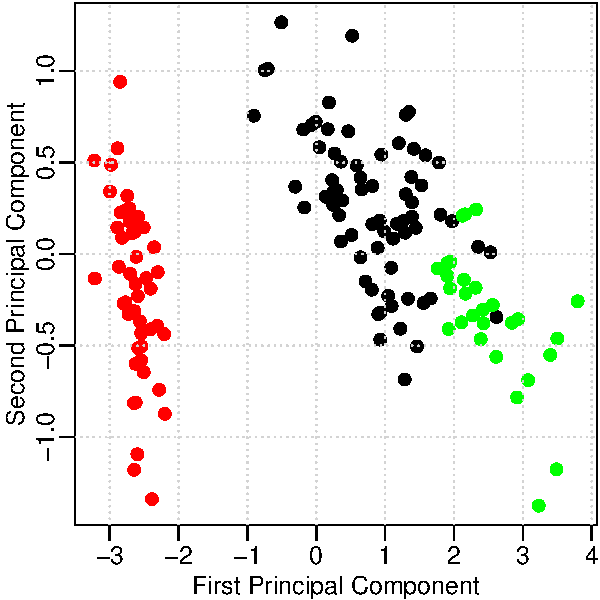
\includegraphics[width=0.60\linewidth]{images/iris_3_clusters.pdf}
  \caption{The resulting clusters for $\hat{\theta}=2.5$ corresponding to three clusters.  While not perfect, it appears that the sequential-forward algorithm does start to differentiate between the nearby classes \emph{Versicolor} and \emph{Virginica}.}
\end{figure}

\subsection{R source code :}

\Rexternal{../src/iris.r}

\end{multicols*}

\newpage

\section{E.~coli data :}

\begin{figure}[H]
  \centering
    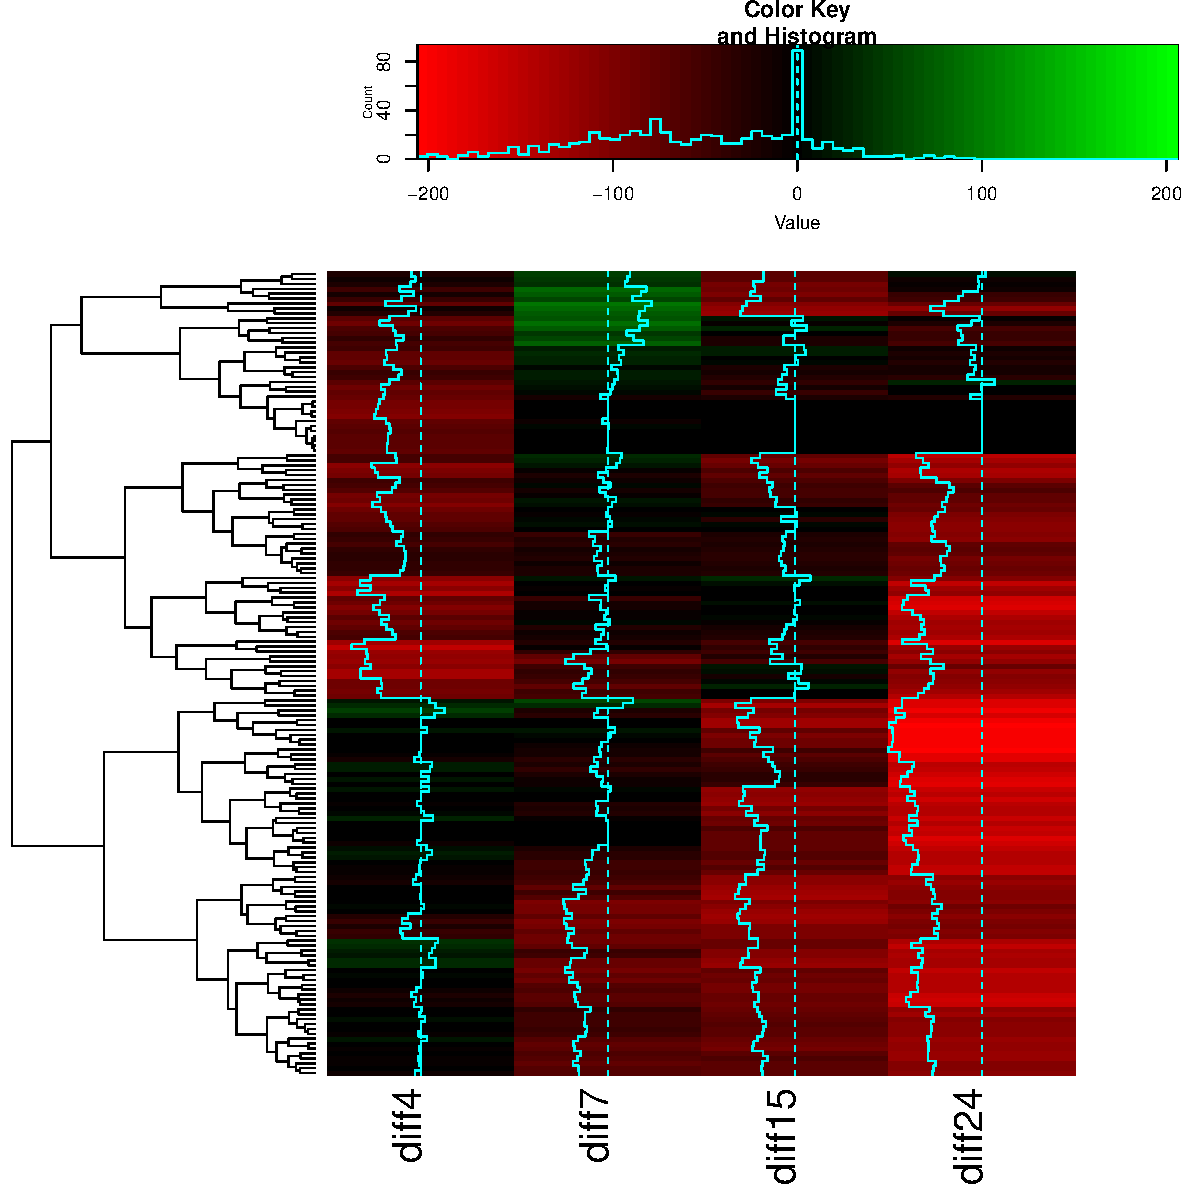
\includegraphics[width=0.95\textwidth]{images/ecoli_heat.pdf}
  \caption{Gene expression samples of E.~coli taken at $t=$4,7,15, and 24 hours, where each row represents a gene's expression profile, i.e., the extent to which the corresponding gene is expressed in biofilm vs.~suspension.  The rows are ordered by cluster hierarchy.}
\end{figure}

\begin{figure}[H]
  \centering
    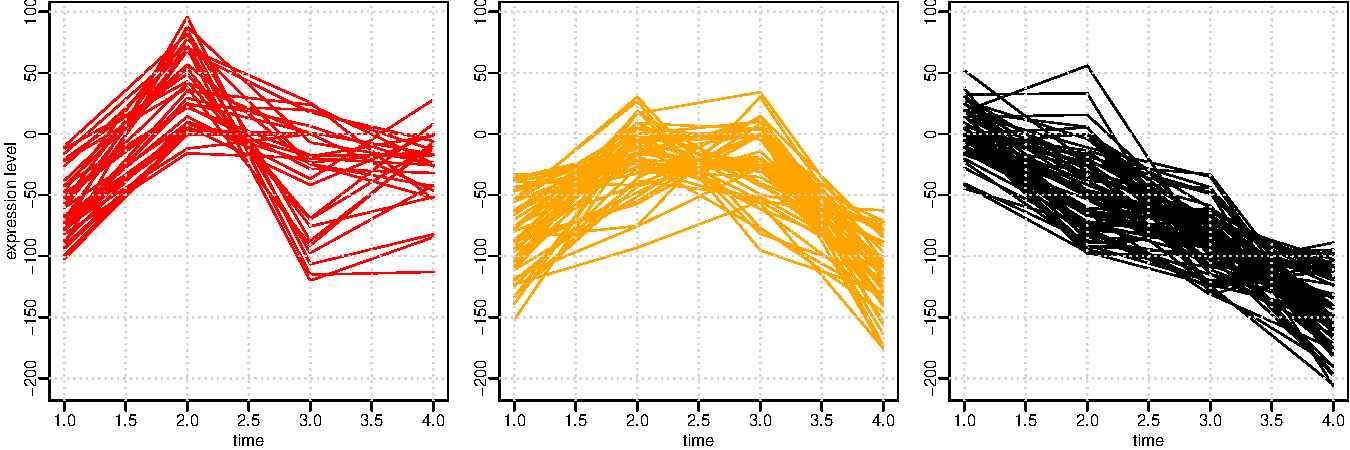
\includegraphics[width=0.95\textwidth]{images/ecoli_lines.pdf}
  \caption{The individual three clusters derived as in Figure 7.  It appears that one cluster exhibits oscillatory behavior (left), one goes up and then back down (middle), and one decreases (right).}
\end{figure}

\begin{multicols*}{2}

\begin{figure}[H]
  \centering
    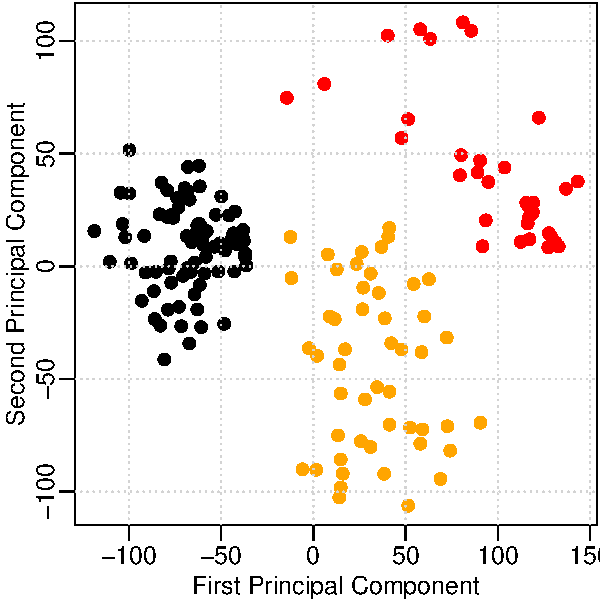
\includegraphics[width=0.8\linewidth]{images/ecoli_pca.pdf}
  \caption{The E.~coli data projected onto the first two principle components, colored by hierarchical clustering.  It appears that there are indeed three distinct clusters here!}
\end{figure}

\vfill
\columnbreak

\subsection{R source code :}

\Rexternal{../src/ecoli.r}

\end{multicols*}



\end{document}


